\section{Track Finding Processor Architecture}\label{sec:tf-arch}
The TFP (Fig.~\ref{fig:TFP}) consists of four self-contained components:
\begin{itemize}
\item {\bf Geometric Processor (GP)} - responsible for pre-processing the stubs from the DTC.
\item {\bf Hough Transform (HT)} - a highly panellised initial coarse track finding.
\item {\bf Kalman Filter (KF)} - cleans tracks, precisely fits helix parameters and removes fake tracks.
\item {\bf Duplicate Removal (DR)} - a final pass filter that uses the precise fit information to remove duplicate tracks generated by the \HT.
\end{itemize}

\begin{figure}[!h]
\centering
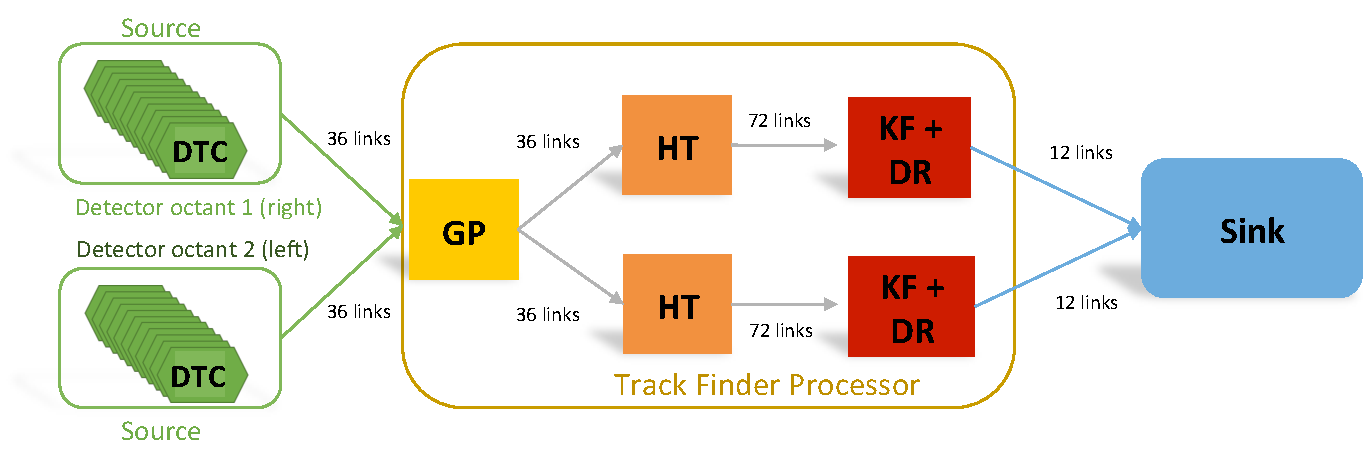
\includegraphics[width=0.78\textwidth]{figs/demoslice/demoslice1.pdf}
% where an .eps filename suffix will be assumed under latex,
% and a .pdf suffix will be assumed for pdflatex; or what has been declared
% via \DeclareGraphicsExtensions.
\caption{The four self-contained logical components of the Track Finding Processor, where each block represents a single FPGA. The two FPGAs for the two detector octant sources and the sink FPGA and the optical links between all components are also shown.}
\label{fig:TFP}
\end{figure}

\subsection{Geometric Processor}
Each GP performs two tasks, firstly the conversion of the 48-bit DTC stubs into a 64-bit format extended format that is used to reduce the HT processing load and the assignment of stubs to thirty six sub-sectors, two sub-sectors in $\phi$ and eighteen in $\eta$ (where $\eta$ is the pseudo-rapidity). This division of the processing octants simplifies the task of the downstream logic required, allowing the track finding to be carried out independently and in parallel within each sub-sector. The relatively fine $\eta$ binning ensures that any track found by the \rphi HT is consistent in the \rz plane. Stubs compatible with more than one sub-sector, usually due to track curvature in $\phi$ are duplicated. The routing of stubs to sub-sectors occurs in three stages: a rough $\eta$ sorting into six bins, a fine $\eta$ sorting into three bins and a $\phi$ sorting into two bins. Each block in this router is highly reconfigurable and can easily be adapted to any alternative sub-sector definition.

\subsection{Hough Transform}
The Hough Transform algorithm is a widely used means of detecting geometric features in digital image processing \cite{HT}. It is used to find primary charged particles with \pT > 3\GeV in the \rphi plane. Within the tracking volume, permeated by a homogeneous 3.8T magnetic field ($B$), a radius of curvature ($R$) can be described as a function of its\pT and charge $q$:

\begin{equation}
R = \frac{\pt}{0.003\,qB} \;.
\label{eq:R}
\end{equation}

Assuming, to first order, that $R$ is constant, by neglecting energy losses such as through multiple scattering, and that only primary tracks from or near the primary interaction point are considered (other such tracks are not typically relevant to the L1 trigger), a stub with coordinates ($r$,$\varphi$) is related to $R$ by:

\begin{equation}
\frac r{2\,R} = \sin\left(\varphi-\phi\right)
\label{eq:stub_R}
\end{equation}

where $\phi$ is the angle of the track in the transverse plane at the origin \cite{markthesis}. For large \pT (> 3\GeV) and thus large $R$, the small angle approximation can be used. Combining Eq.~\ref{eq:R} and Eq.~\ref{eq:stub_R}, one produces the key formula showing the transformation from stub positions to straight lines in the track parameter plane (Hough-space):

\begin{equation}
\phi = \varphi - \frac{0.0015\,qB}{\pt}\cdot r \;.
\label{eq:localHT}
\end{equation}

The point of intersection of these lines in Hough-space would therefore correspond to a circle in the \rphi plane which is consistent with the primary interaction point and all stubs involved.

As the line gradients in Hough-space is given by the radius of the stubs, they will always be positive, the stub radius is transformed to $r_{58} = r - 58cm$ in order to utilise a larger phase space, which leads to fewer \textit{fake} (in that the found track does not match to a simulated particle) and duplicated tracks.

Given that $R$ for the lowest \pT track (3\GeV) to be considered is greater than the outer radius of the tracking detector ($r$ = 1.2m), all relevant particles are expected to traverse through at least six barrel layers or endcap disks. The threshold for the identification of a track candidate however, is set at a minimum of five detector layers or disk in order to allow for detector or readout inefficiencies. This threshold can be further reduced to four layers to account for the reduced geometric coverage between $0.89 < \eta < 1.16$ or for dead detector layers or disks.

\subsubsection{Implementation}
A two stage fully pipelined design has been implemented in FPGA firmware, firstly the HT array is filled before the reading out of the HT track candidates. 

The \textit{Book Keeper} (Fig.~\ref{fig:implementationHT}) unpacks stub data from the input links and propagates stubs from one \textit{Bin} to the next each clock cycle, before the track candidate stubs are returned to the Book Keeper and transmitted downstream. Each Bin (Fig.~\ref{fig:implementationHT}) represents a $q/\pT$ column in the HT array. Using the left and right boundary results of the \HT calculation, it is determined if the stub crosses two $\phi$ rows and if so, it is duplicated and processed at the next available gap in the data stream. The stubs are sorted into the sixty four $\phi$ rows in the Track Builder's memory and if there are $\phi$ cells which meet the threshold requirement on the minimum number of hit layers/disks, the row is marked for readout. The \textit{Hand Shake} component is responsible for shifting the track candidate stubs from bin to bin until there are no further stubs, before enabling the reading out of the Track Builder.

\begin{figure}[!t]
\centering
\includegraphics[width=0.57\textwidth]{figs/tk-arch/ht/bookKeeper.pdf}
\includegraphics[width=0.37\textwidth]{figs/tk-arch/ht/bin.pdf}
% where an .eps filename suffix will be assumed under latex,
% and a .pdf suffix will be assumed for pdflatex; or what has been declared
% via \DeclareGraphicsExtensions.
\caption{Overview of a \textit{Book Keeper} (left) and a \textit{Bin}. Internal components are shown as boxes and data paths as lines, where arrows indicate the direction of data flow}
\label{fig:implementationHT}
\end{figure}

As the Book Keeper receives only one stub per clock cycle, thirty six arrays per octant are required to process the large number of stubs associated with each event at high pileup. Each array (or Hough Segement) corresponds to one sub-sector from the GP, covering thirty two columns in \qpt and a sixty four row sub-range in $\varphi$.

A more detailed description of the firmware implementation of the \HT for the demonstrator system is discussed in \cite{IEEE} and \cite{TmttNote}.

\subsection{Kalman Filter}
Coarse \rphi helix parameters out of the \HT are used as the initial variables for track finding, with the segment assignment also providing a good seed value. Given that in simulation over half the track candidates from by the HT are considered to be \textit{fake} or contain at least one stub associated with another particle, a Kalman Filter is used to both remove these incorrect stubs and reject fake tracks. 

In addition to the advantages of the Kalman filter for track reconstruction discussed by Fr{\"u}hwirth in \cite{Fruhwirth:1987fm}, the algorithm has several aspects making it suitable for FPGA implementation compared to global track fitting methods, namely the matrices:

\begin{itemize}
\item {are small.}
\item {are size independent of the number of measurements.}
\item {only involve the inversion of a small matrix.}
\end{itemize}

The initial estimate, or \textit{state}, of the track parameters and their uncertainties are updated by the KF iteratively applying stubs to update the state following the Kalman formalism, decreasing the uncertainty in the state. The relative uncertainties in the state and their associated measurements control parameter adjustment. Missing layers can be skipped due to missing or incorrect stubs and multiple stubs on the same layer are each propagated and ranked, with up to the four best states being kept and presented to a final state selector.

As the final fit is always performed after a fixed period of time, there is no truncation in the traditional sense as all candidates will be read out, although events such as dense jets with many candidates	and stubs per candidate will only be partially filtered.

A greater in-depth discussion of the mathematics and implementation of online track reconstruction using Kalman Filters on FPGAs in \cite{SSummers}.

\subsection{Duplicate Removal}
At the input to the DR, over half of the track candidates are unwanted duplicate tracks created by the HT. Naively one would expect the need to compare pairs of tracks to see if they are the same as each other, but by understanding how the HT produces these duplicate tracks a more elegant and subtle DR algorithm can be used. This approach is illustrated in Fig.~\ref{fig:DR}, where five stubs (blue lines in Hough Space) produces three candidates (green and yellow cells). As all three candidates contain the same stubs, they will be fitted with identical helix parameters in the same cell (the yellow cell) regardless of the original HT cell. The algorithm accepts only tracks whose fitted parameters are consistent to those that the HT found them in initially. There is however, a small subtlety, given that the algorithm eliminates unique tracks whose fitted parameters were not consistent, which results in the loss of a few percent of efficiency. By performing a second pass through the rejected tracks and rescuing those which are unique the lost efficiency can be recovered.


\begin{figure}[!h]
\centering
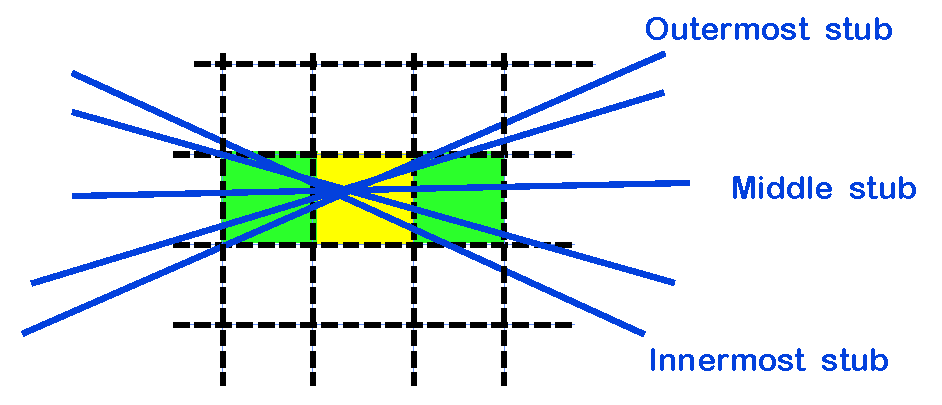
\includegraphics[width=0.80\textwidth]{figs/tk-arch/dr/A50_algo.pdf}
% where an .eps filename suffix will be assumed under latex,
% and a .pdf suffix will be assumed for pdflatex; or what has been declared
% via \DeclareGraphicsExtensions.
\caption{Illustration of how duplicates are formed by the \rphi \HT.}
\label{fig:DR}
\end{figure}

\subsubsection{Implementation}
A minimum resource usage strategy has resulted in firmware that can be integrated in the same board as the KF. Tracks which are consistent in both HT and KF space are marked in a matrix, which allows only one track per cell, are forwarded to the output. Tracks which are not consistent and not yet in the matrix are kept in a FIFO until a certain time threshold is reached, then, if the tracks point to a still unmarked cell, they are marked in the matrix and forwarded to the output. 

Two matrices are used in an interleaving fashion as a complete reset is required before processing tracks from the following event. Additionally, two FIFOs (one per matrix) are required to store the addresses that were marked and thus require to be cleared in the event, therefore resulting in there being always one active and one resetting matrix.